\section{Theory: Neural dynamics}
\label{sec:Neuron}
\begin{itemize}
\item Multicompartmental modeling
\item Cable equation
\item No current monopoles - trick needed for point neurons
\end{itemize}

Modelling of neurons is at the core of computational neuroscience, and the topic has been treated in detail in several text books (see e.g., \cite{johnston1994foundations, KockSegev1998, Koch1999, Hille2001, Dayan2005, Sterratt2011}). We therefore only give a brief introduction to it here. 

Most simulations of extracellular potentials are based on biophysical multicompartmental neuronal models, which are typically based on a formalism similar to that used in the celebrated model by Hodgkin and Huxley \cite{Hodgkin1952}. In models based on
a Hodgkin-Huxley-type formalism, a neuron is characterized by (i) its morphology, and (ii) its membrane mechanisms. In a multicompartmental model\index{multicompartment modelling}, the morphology of the real neuron (Fig. \ref{Neuron:fig:multicomp}A) is represented as a discretized set of compartments connected by resistors (Fig. \ref{Neuron:fig:multicomp}B). In such a model there are two categories of currents which together determine the membrane potential dynamics of the neuron (Fig. \ref{Neuron:fig:multicomp}C). These are the currents that run intracellularly between compartments (yellow arrows), and the transmembrane currents (green arrows). Once all the currents are characterized, the dynamics of the membrane potential can be computed by demanding that the sum of currents into a given compartment is zero (Kircchoff's current law). 

\begin{figure}[!ht]
\begin{center}
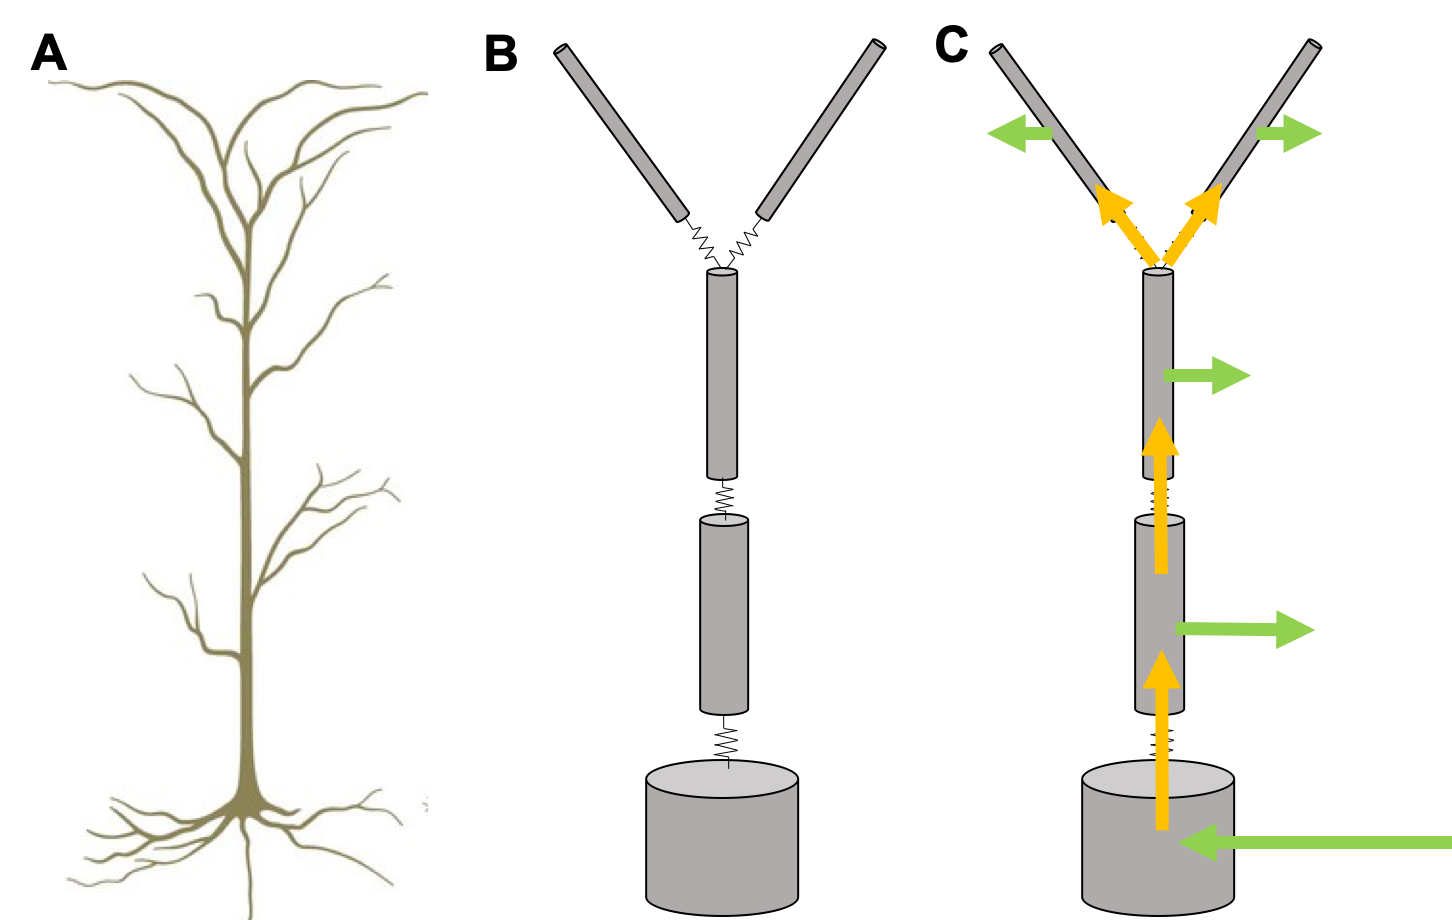
\includegraphics[width=0.6\textwidth]{Figures/Neuron/Multicomp.png}
\end{center}
\caption{\textbf{Multicompartmental modelling.} 
}
\label{Neuron:fig:multicomp}
\end{figure}

Below, we first present a framework for modeling the transmembrane currents in a single compartment (subchapter called "Membrane currents"), and next show how a number of such compartments can be connected together to a multicompartment model (subchapter called "Morphology").


\subsection{\blue{Membrane currents}}
In Hodgkin-Huxley type models, the membrane typically includes three autonomous classes of transmembrane currents, normally represented as current densities (unit mA/cm$^2$). These are (i) a capacitive current density ($i_c$), (ii) a the leakage current density ($i_L$), and (iii) a the current density through active ion channels ($i_x$), of which there may be several different kinds ($x$ is an index). In addition, a neuron may receive  (iv) external stimuli ($i_{stim}$) either through synaptic currents or experimental current injections. In the case where the neuron is modeled as a single compartment, the net transmembrane current must be zero, so that:

\begin{equation}
i_c + i_L + \sum_x{i_x} +  i_{stim} = 0.
\label{eq:singlecomp_zerosum}
\end{equation}
Below, we define the various currents that go into this equation.

\subsubsection{\blue{Capacitive current}}
The capacitive current density,
\begin{equation}
i_c = c_m \frac{d\phi_m}{dt},
\label{eq:HHcap}
\end{equation}
represents the charging up of the membrane potential $\phi_m$ due to a charge density accumulating on the outside of inside of the capacitive membrane. Here, $c_m$ is the specific membrane capacitance. In the HH-model, $c_m$ had the value
1 $\mu$F/cm$^2$, and this value seems to be representative for most neurons.  An illustration of how to interpret the capacitive current is given in Fig. \ref{Neuron:fig:capacitive_currents}. 

\begin{figure}[!ht]
\begin{center}
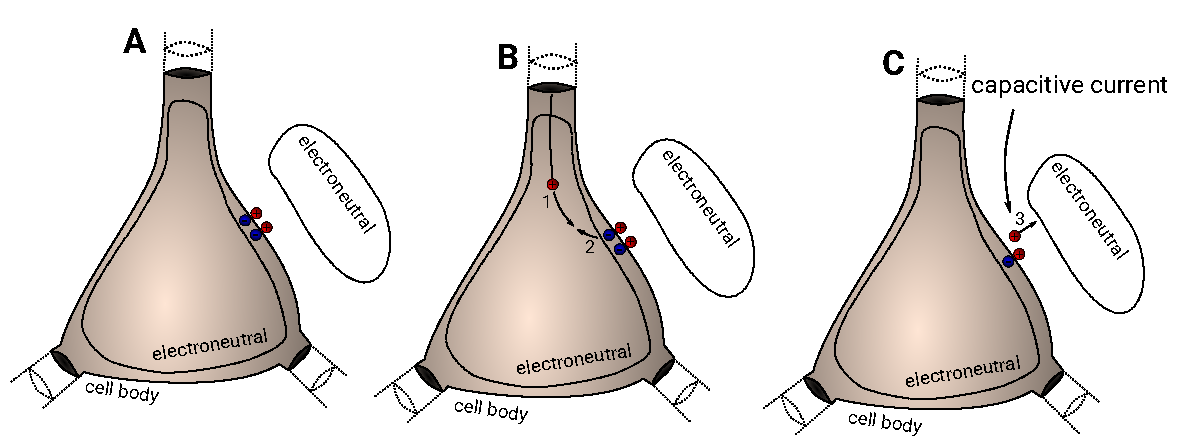
\includegraphics[width=0.8\textwidth]{Figures/Neuron/capacitive_currents.pdf}
\end{center}
\caption{\textbf{Capacitive currents are important for current conservation.}  (\textbf{(A)}) The extracellular and intracellular bulk solutions are essentially electroneutral, and the only region where there is a nonzero charge density is in thin Debye layers around the capacitive membrane. The capacitive current is not due to ions crossing the membrane, but due to ions piling up on either side of it, separating a charge density $\rho$ and a charge density $-\rho$, giving rise to a membrane potential of $\phi_m = \rho/c_m$. An outward capacitive current could correspond to an anion leaving the membrane on the inside (\textbf{(B)}), which will coincide with a cation leaving the membrane on the outside (\textbf{(C)}). Thus, capacitive membrane currents do give rise to electrical ionic volume currents both in the intra- and extracellular space.
}
\label{Neuron:fig:capacitive_currents}
\end{figure}


\subsubsection{\blue{Leakage current}}
The leakage current density is given by
\begin{equation}
i_L = \bar{g}_L (\phi_m - E_L),
\label{eq:HHleak}
\end{equation}
where $\bar{g}_L$ (mS/cm$^2$) is the leak conductance (the bar indicates that it's a constant). The factor $(\phi_m - E_L)$ (mV) is often called the driving force, and $E_L$ the leak reversal potential. The biophysical origin of the reversal potential is explained later (see SECTION). For now, we will simply think of $E_L$ as the "target potential" that the leakage current will strive to drive the membrane towards. In reality, the leakage current is not a single current, but represents an orchestra of physiological processes that together will drive the membrane potential towards $E_L$. Together, the capacitive current and the leakage current determine the passive properties of the membrane. If the neuron were to include only these two currents, it could be well modeled as an RC-circuit, and RC-neuron models are often used to simulate the subthreshold dynamics of neurons (Fig. \ref{Neuron:fig:RC}). 

\begin{figure}[!ht]
\begin{center}
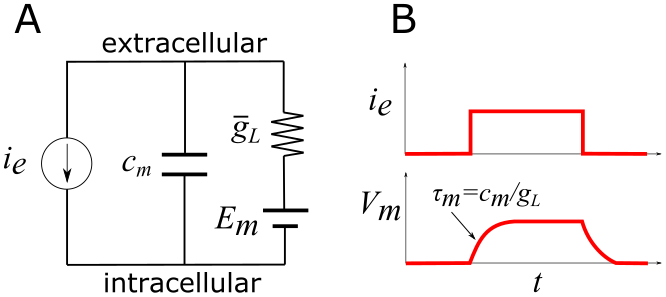
\includegraphics[width=0.8\textwidth]{Figures/Neuron/RCneuron.png}
\end{center}
\caption{\textbf{RC-neuron.}  A neuron model containing only a capacitive and a leakage current can be represented as an RC-circuit ($R = 1/g_L$). In the illustration, the neuron is given a current injection $I$ and responds by charging up the membrane. When the input is terminated, the membrane potential will return to the value $E_L$.
}
\label{Neuron:fig:RC}
\end{figure}

In the RC-model, $E_L$ will be identical to the resting potential of the neuron. In the more general models, which also include active ion channels (see below), the resting potential will still tend to be close to $E_L$, but will typically not be identical to $E_L$, as there some of the active ion channels can be partially open during rest, and thus affect the resting potential. For example values, see the parameters used in the original Hodgkin-Huxley model (Table \ref{tab:HH}).

\subsubsection{\blue{Active ion channels}}
In addition to $I_c$ and $I_L$, biophysical neuronal models typically include a number of active ion channels. When based on a Hodgkin-Huxley type formalism, current through an active an active ion channel $x$ is modeled as:

\begin{equation}
I_x = \bar{g}_x m_x^{\alpha} h_x^{\beta}(V-E_x)
\label{eq:HHform}
\end{equation}

Here, $\bar{g}_x$ (mS/cm$^2$) denotes the conductance when all channels of type $x$ are fully open (the bar indicates that it's a constant), while $E_x$ (mV) is the reversal potential for the ion species that travels through the channel. In analogy with the leak reversal potential, we may think of $E_x$ as the target potential that the current through ion channel $x$ will strive to drive the membrane potential towards. The intrinsic membrane potential dynamics is thus due to the competition between various currents that try to drive it towards their respective reversal potentials. We note that the current density $i_x$ does not represent the current through a single ion channel, but a large number of channels of the same type $x$. 

Active ion channels differ from the passive leakage channel in that their total conductance, $\bar{g}_{x} m^{\alpha} h^{\beta}$, will vary with time due to the so-called gating variables, in eq. \ref{eq:HHform} denoted $m$ and $h$. These determine the dynamics of how the ion channel activates or deactivates (opens or closes). Here, $m$ and $h$ represent two different types of gates, which have different dependencies in terms of what causes them to open/close. The exponents $\alpha$ and $\beta$ indicate that a channel $x$ may have several copies of each type of gate. The values of $m$ and $h$ interpret as the fraction of the gates of the various types that are open, and the values are thus numbers between zero (all gates in the closed state) and one (all gates in the open state). For an ion channel to be open, all its gates must be in the open state. The product $m^{\alpha} h^{\beta}$ thus interprets as the fractions of ion channels that are open, so that the ion channel conductance is given by the product $\bar{g}_x m_x^{\alpha} h_x^{\beta}$.

For voltage-gated ion channels, the the dynamics of the gating variables are described by kinetics equations on the form:
\begin{equation}
\frac{dx(\phi_m,t)}{dt} = \frac{x_{\infty}(\phi_m) - x}{\tau_x(\phi_m)},  \, \text{for } x = \{m,h\}.
\label{eq:HHgate}
\end{equation}
Here, the steady state activation $x_{inflty}(\phi_m)$ and activation time constant $\tau_x(\phi_m)$ (ms) are functions of the membrane potential, and these must be determined experimentally for each individual ion channel type. We do not go into these experimental issues here. 

The same kind of formalism can also be applied to ligand gated ion channels, i.e., channels that instead of opening and closing as a function of the membrane potential $\phi_m$, open or close as a function of a concentration of some ligand. The most common ligand gated channels in the brain are Ca$^{2+}$ gated ion channels, i.e., channels with gate opening controlled by the intracellular Ca$^{2+}$ concentration ($[Ca^{2+}]_i$), where:

\begin{equation}
\frac{dx(\phi_m,t)}{dt} = \frac{x_{\infty}([Ca^{2+}]_i) - x}{\tau_x([Ca^{2+}]_i)},  \, \text{for } x = \{m,h\}.
\label{eq:HHgateCa}
\end{equation}


\subsubsection{\orange{Stimulus currents and synapses}}
Finally, the stimulus current in Eq. \ref{eq:singlecomp_zerosum}, can be represent any external stimulus that a neuron receives. Typically, it is either taken to represent an experimental current injection, 

\begin{equation}
i_\text{inj}(x)= 
\begin{cases}
    constant, & \text{if } t_{start} > t > t_{end} \\
    0,              & \text{otherwise}
\end{cases}
\label{eq:injected}
\end{equation}
or a synaptic input. Synapses come in many forms, and they can be either inhibitory (making the receiving neuron less likely to fire) or excitatory (making the receiving neuron more likely to fire). The most common synapses are chemical synapses, which are normally modeled more or less like an ion channel:
\begin{equation}
I_\text{syn}(t) = g_\text{syn}(t) \big( \phi_m(t)-E_\text{syn} \big), 
\label{eq:chemicalsynapse}
\end{equation}
where $E_\text{syn}$ is the reversal potential of the synapse, and $g_\text{syn}(t)$ the conductance. Unlike for ion channels, which are often voltage or calcium activates, the synapse is activated by neurotransmitters from the pre-synaptic cell. As the response is quite stereotypical (i.e., the same every time a synapse is activated), it is common to model $g_\text{syn}(t)$ as a constant $\bar{g}_\text{syn}$ multiplied with a temporal kernel determining the opening and closing of a synapse set off at an activation time $t_s$. Typical choices for $g_\text{syn}(t)$ are: 

\begin{align}
&\text{(i) exponential decay:} \;\; g_\text{syn}(t) = \bar{g}_\text{syn} e^{-(t-t_\text{s})/\tau}\, \Theta(t-t_\text{s}) \\
&\text{(ii) $\alpha$-function:} \;\; g_\text{syn}(t) = \bar{g}_\text{syn} \frac{t-t_\text{s}}{\tau} e^{-(t-t_\text{s})/\tau} \, \Theta(t-t_\text{s}) \\
&\text{(iii) $\beta$-function:} \;\; g_\text{syn}(t) = \bar{g}_\text{syn} \frac{\tau_1 \tau_2}{\tau_1-\tau_2} 
\Big( e^{-(t-t_\text{s})/\tau_1} - e^{-(t-t_\text{s})/\tau_2} \Big) \, \Theta(t-t_\text{s}) \\
& \text{(iv)} g_\text{syn}(t) = \bar{g}_\text{syn} \frac{e^{-(t-t_\text{s})/\tau_1} - e^{-(t-t_\text{s})/\tau_2}} {1+\mu [\text{Mg}^{2+}] e^{-\gamma \phi_m} } \, \Theta(t-t_\text{s}),
\label{eq:synapseforms}
\end{align}
where $\Theta(t)$ is the (Heaviside) unit step function: $\Theta(t \ge 0)=1$,   $\Theta(t< 0)=0$. Simple waveform (cf., (i)--(iii) above) typically used for AMPA  and GABA receptors, while the waveform (iv), is mainly relevant for NMDA-receptors, 
where the conductance is influenced by membrane voltage and concentration of extracellular magnesum. In all these equation, $the \tau$'s and the $\gamma$ are parameters that determine the time course of the synapse opening, and must be tuned to experimental data. 

Chemical synapses may be plastic, meaning that their maximum conductance $\bar{g}_\text{syn}$ can vary with time, depending on the spiking history of the neuron. Synaptic plasticity is the mechanism for learning and memory formation. We do not go further into this topic here. 

In addition to having chemical synapses, some neurons may also be connected directly by electrical synapses called \underline{gap junctions}, where the current from one neural process into the other is simply a function of the voltage difference between them and the conductance: 

\begin{equation}
i_\text{gap}=g_\text{gap} (\phi_{m2}-\phi_{m1})
\label{eq:gapjunction}
\end{equation}


\subsubsection{\orange{The Hodgkin-Huxley model}}
\ghnote{Maybe make this a box.}
To give an example of a model with active ion channels, we here list up the equations for the original Hodgkin-Huxley model. Compared to modern biophysically detailed neuron models, it is relatively simple in that it only contains two (voltage-gated) active ion channels, a Na$^+$ with three activation gates ($m^3$) and one inactivation gate ($h$), as well as a K$^+$ channel with four inactivation gates $n^4$:
\begin{equation}
c_m \frac{d\phi_m}{dt} = -\bar{g}_L(\phi_m-E_L) - \bar{g}_{Na} m^3 h (\phi_m - E_{Na}) - \bar{g}_{K} n^4 (\phi_m - E_{K}).
\label{eq:HHfull}
\end{equation}
The two active ion channels are together responsible for action potential generation. In eq. \ref{eq:HHfull}, $\bar{g}_{Na}$ and $\bar{g}_K$ are the conductances for fully open channels, while $E_{Na}$ and $E_{K}$ are the Na$^+$ and K$^+$ reversal potentials. Like we defined in eq. \ref{eq:HHgate}, the gating kinetics is given by: 
\begin{equation}
\frac{dx(\phi_m,t)}{dt} = \frac{x_{\infty}(\phi_m) - x}{\tau_x(\phi_m)},  \, \text{for } x = \{m,h,n\}.
\label{eq:HHgates}
\end{equation}
The experimentally determined functions for $x_{infty}(\phi_m)$ and $\tau_x(\phi_m)$, and all model parameter values are given in Table \ref{tab:HH}. An electric circuit representation of the HH model is depicted in Fig. \ref{Neuron:fig:HHcircuit}

\begin{table}[h!]
\begin{center}
\caption{The Hodgkin-Huxley model}
\label{tab:HH}
    \begin{tabular}{l}
    \hline
    $x_{\infty}(\phi_m) = \frac{\alpha_x(\phi_m)}{\alpha_x(\phi_m) + \beta_x(\phi_m)}$ for $x = m,n,h$ \\ \hline
    $ \alpha_n = \frac{0.01 \mathrm{ms}^{-1} \phi_m+55 \mathrm{mV}}{1-e^{-(\phi_m+55 \mathrm{mV})/10 \mathrm{mV}}}$  \\ \hline
    $ \beta_n = 0.125 \mathrm{ms}^-1 e^{-(\phi_m+65 \mathrm{mV})/80 \mathrm{mV}} $  \\ \hline
    $ \alpha_m = \frac{0.1 \mathrm{ms}^{-1} \phi_m+ 40 \mathrm{mV}} {1-e^{-(\phi_m+40 \mathrm{mV})/10 \mathrm{mV}}}$  \\ \hline
    $\beta_m = 4 \mathrm{ms}^{-1} e^{-(\phi_m+65  \mathrm{mV})/18 \mathrm{mV}} $  \\ \hline
    $\alpha_h = 0.07 \mathrm{ms}^{-1} e^{-(\phi_m+65 \mathrm{mV})/20 \mathrm{mV}}$  \\ \hline
    $\beta_h = \frac{1 \mathrm{ms}^{-1}}{1+e^{-(\phi_m+35 \mathrm{mV}))/10 \mathrm{mV})}} $  \\ \hline
    $c_m = 1.0 \mu $F/cm$^2$ \\ \hline
    $\bar{g}{Na} = 120\times 10^{-9}$ m$^2$/s\\ \hline
    $\bar{g}_{K} = 36$ mS/cm$^2$ \\ \hline
    $\bar{g}_{L} = 0.3$ mS/cm$^2$ \\ \hline
    $E_{Na} = 50$ mV \\ \hline
    $E_{K} = -77$ mV \\ \hline
    $E_{L} = -54.4$ mV \\ \hline
    \end{tabular}
\end{center}
\end{table}

\begin{figure}[!ht]
\begin{center}
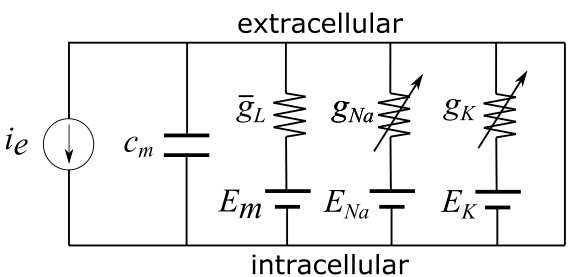
\includegraphics[width=0.8\textwidth]{Figures/Neuron/HHmodel.png}
\end{center}
\caption{\textbf{Hodgkin Huxley model.}
}
\label{Neuron:fig:HHcircuit}
\end{figure}


\subsubsection{\orange{Reversal potentials}}
\ghnote{Maybe move this as part of the the "assumptions" subsection at the end?}
A prerequisite for having transmembrane currents in neurons is that the intra- and extracellular solutions contain different ionic compositions. Neurons have a set of homeostatic mechanisms that make sure that it stays that way. The perhaps most important of these is the ATPase pump, which uses energy to pump K$^+$ ions into the neuron and Na$^+$ ions out, and as a result, the intracellular space is comparatively rich in K$^+$, while the extracellular space is comparatively rich on Na$^+$. Typical values of ion concentrations of the main charge carriers inside and outside neurons are given in Table \ref{table:ion-concentrations}.

\begin{table}[h]
\centering
\caption{Major charge carrier concentrations inside/outside a typical mammalian neuron. Example values taken from \cite{Wu2019}, but may vary with species and brain regions. Nernst potentials were computed from Eq. \ref{eq:revpots} assuming a body temperature of 309.15 K.}
\label{table:ion-concentrations}
{\begin{tabular}{lccccc}\toprule
						    & 	K$^+$	&	Na$^+$	&	Mg$^2+$	  &	Cl$^-$	&	Ca$^{2+}$	 \\ \midrule
Inside (mM)				    & 140		&		10	&		0.5	&	10		&  	10$^{-4}$	  	\\
Outside (mM)			           & 5			&		145	&		2	&	110 		&		2		  	\\
Nernst potential (mV)		    &	-89		&	    	+71	&		+19	&	-64		&		+132 		  	\\
\bottomrule
\end{tabular}}{}
\end{table}

Ion channels are pores in the membrane, some of which are selectively permeable only to specific ions. For example, when a Na$^+$ channel opens, only Na$^+$ ions will pass through it, and they will diffuse from the extracellular space, where the Na$^+$ concentration is highest, and into the neuron. As this diffusive process transfers charged ions into the neuron, it will charge up the membrane potential. The membrane potential will in turn evoke an electrostatic force on the Na$^+$ ions, causing an electrical drift of Na$^+$ in the opposite direction. The ionic reversal potential is defined as the potential at which the electrical drift current and diffusive current of a given ion species are in an equilibrium where they are equal in magnitude but oppositely directed. It can be calculated from the Nernst-Planck equation for electrodiffusion. If we approximate the problem as one-dimensional (in the $z$-direction, perpendicular to the membrane), the Nernst-Planck equation for an ion species $k$ is:
%%%%
\begin{equation}
j_k = j_{k,\text{diff}} + j_{k,\text{drift}} 
=  - P_k \Big(\frac{d[k]}{dz} +  \frac{Fz_k}{RT}  [k] \frac{d\phi}{dz} \Big), 
\label{eq:NP1D}
\end{equation}
%%%%
where the first term is Fick's law for the diffusive flux density along the concentration gradient, and the second term is the electrical drift along the voltage gradient. Here, the membrane permeability ($P_k$) to ion $k$ has replaced the diffusion constant in a free solution ($D_k$) which appears in the more common form of the Nernst-Planck equation. Furthermore, $z_{k}$ is the valency of ion species $k$, $R = 8.314$ J mol$^{-1}$K$^{-1}$ is the gas constant, $F = 96485.3365$ C/mol is Faraday's constant, and $T$ is the absolute temperature (K). The reversal potential (also called the Nernst-potential) is found by solving for when there is no net flux, i.e., when  $j_{k,\text{diff}} = - j_{k,\text{drift}}$:

\begin{equation}
\frac{1}{[k]} \frac{d[k]}{dz} = - \frac{Fz_k}{RT}  \frac{d\phi_m}{dz}.
\end{equation}
We may multiply both sides by $dz$ and re-arrange this to get:
\begin{equation}
-d\phi = \frac{RT}{Fz_k}  \frac{d[k]}{[k]}.
\end{equation}
Now we may integrate from the inside to the outside of the membrane:
\begin{align}
-\int_{\phi_{\text{in}}}^{\phi_{\text{out}}}  dV &= \frac{RT}{Fz_k}  \int_{[k]_{\text{in}}}^{[k]_{\text{out}}} \frac{d[k]}{[k]} \rightarrow \\
\phi_{\text{in}}-\phi_{\text{out}} &= \frac{RT}{Fz_k} ln \frac{[k]_{\text{out}}} {[k]_{\text{in}}} \rightarrow \\
E_k & =  \frac{RT}{Fz_k}  ln \frac{[k]_{\text{out}}} {[k]_{\text{in}}} 
\label{eq:revpots}
\end{align}
where the last equality follows from the definition of $E_k$ as the membrane potential $\phi_{\text{in}}-\phi_{\text{out}}$ for which the the net flux (in Eq. \ref{eq:NP1D}) is zero. Eq. \ref{eq:revpots} was used to compute the reversal potentials listed in Table \ref{table:ion-concentrations}. 

Based on Eq. \ref{eq:NP1D} and a few assumptions, it has been shown that a membrane current is well described by the Goldman-Hodkgkin-Katz equation (see e.g., \cite{johnston1994foundations}):

\begin{equation}
I_\text{k} = P_k z_k F \frac{z_k F \phi_m}{R T} \Big( \frac{[k]_\text{in}-[k]_\text{out} e^{-z_k F \phi_m/RT}} {1-e^{-z_k F \phi_m/RT}} \Big), 
\label{eq:GHK}
\end{equation}
The transmembrane currents used in the HH type formalism (Eq. \ref{eq:HHform}), which are proportional to the driving force $(V-E_k)$, are linearized (sometimes called quasi-Ohmic) versions of the Goldman-Hodkgkin-Katz equation.

Eq. \ref{eq:NP1D} defined the reversal potential for individual ion species, which is relevant for ion specific ion channels. In contrast, the passive membrane has some leakage permeability to all ion species simultaneously. This gives rise to a leak reversal potential $E_L$ (from Eq. \ref{eq:HHleak}), representing the equilibrium condition where the leakages of various ions across the membrane sum to a zero net electrical current. If we assume that only the three most important charge carriers (K$^{+}$, Na$^{+}$ and Cl$^{-}$) contribute, and that they are defined by Eq. \ref{eq:GHK} with leak permeabilities $P_K$, $P_{Na}$ and $P_{Cl}$, it can be shown that they are in equilibrium at the potential:

\begin{equation}
E_L = \frac{R T}{F} 
\ln \frac{P_\text{K} [K]_\text{out}+P_\text{Na} [Na]_\text{out} + P_\text{Cl} [Cl]_\text{in}}
           {P_\text{K} [K]_\text{in}+P_\text{Na} [Na]_\text{in} + P_\text{Cl} [Cl]_\text{out}}.
\end{equation}


%%%%%%%%%%%%%%%%%%%%%%%%%%
\subsection{\blue{Morphology}}
The formalism introduced so far has been for the modeling a neuron as a single compartment. When doing that, one implicitly assumes that the whole neuron is isopotential (same $\phi_m$ evenrywhere). This is generally not true, and especially not in neurons with long and branchy dendrites, where $\phi_m$ can be very different in the soma compared to what it is in the tip of a distal dendrite. Models that account for morphological features of neurons are called multicompartmental models (Fig. \ref{Neuron:fig:multikompisen}A). The neural morphology is then represented as cylindrical compartments connected with resistors, and $\phi_m$ can be computed in each individual compartment. 

\begin{figure}[!ht]
\begin{center}
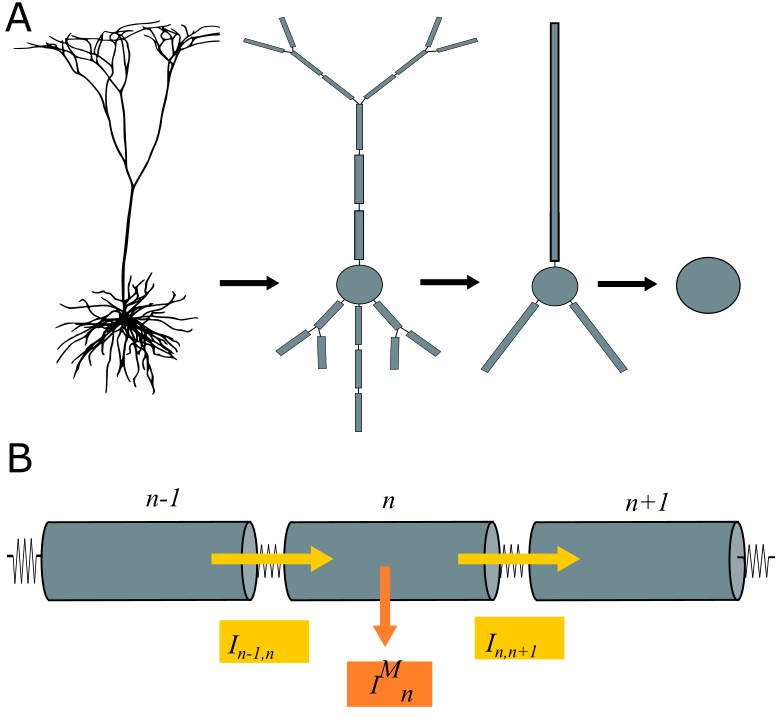
\includegraphics[width=0.7\textwidth]{Figures/Neuron/Multikompis.png}
\end{center}
\caption{\textbf{Multi-compartment model.}
}
\label{Neuron:fig:multikompisen}
\end{figure}

As a simple introduction to the formalism used in multicompartmental models, let us consider a subset of compartments, consisting of three connected cylindrical compartments (Fig. \ref{Neuron:fig:multikompisen}B), and let us for simplicity assume that the three cylinders have the same length ($L$) and diameter ($d$). The two categories of currents that run in this system are (i) the transmembrane currents that we introduced in the previous subsection, all of which we can group together into a total transmembrane current $I^M_j$, and (ii) the axial currents running between the cylindrical compartments ($I_{n-1,n}$ denotes the current from compartment $n-1$ to $n$). 

The dynamics of this system is computed using Kirchhoff's current law, which demands that the sum of currents into a given segment ($n$) should be zero:

\begin{equation}
I_{n-1,n} - I_{n,j+1} - I^M_n = 0
\label{eq:Kirch}
\end{equation}
We note that we calculate with total currents here (unit A), not current densities. The axial currents between two compartments are proportional to the voltage difference between the compartments, as determined by Ohms law:
\begin{eqnarray}
I_{n-1,n} = \frac{\phi_{n-1}-\phi_n}{4 R_a L/(\pi d^2)}, \nonumber \\ 
I_{n,n+1} = \frac{\phi_{n}-\phi_{n+1}}{4 R_a L/(\pi d^2)}.
\label{eq:axialcurrents}
\end{eqnarray}
Here, the denominators represent the axial resistance between two compartments, defined in terms of the axial resistivity $R_a$ ($\Omega$ cm), a material property of the cytosol solution, the cross section area $\pi d^2/4$, and the segment length or travel distance ($L$ (m)). We note that $\phi_n$ is the \emph{intracellular} potential in compartment $n$, but we shall in the reminder of this chapter assume that the extracellular space is isopotential and grounded ($\phi = 0$ there), so that the $\phi_n$ will be identical to the membrane potential in compartment $n$.

The situation becomes more complicated when the connected cylinders are of different length and diameter, and especially at branch points. However, the theory for computing the dynamics in branching structures with varying diameters is well established \cite{Rall1977,Rall1989}, and designated software such as NEURON \cite{Hines1997, Hines2009} automatizes the compartmentalization for the user once the neural morphology is specified. For the reminder of this chapter, we stick with our simplified scenario (Fig. \ref{Neuron:fig:multikompisen}B), as we deem this as sufficient for establishing an understanding of the essentials of morphology modeling. 


%%%%%%%%%%%%
\subsubsection{\blue{Active multicomparmtent models}}
To specify our neuron model further, we write the membrane current as
\begin{equation}
I_n^{cap} + I_n^{ion} + I_n^{leak} + I_n^{stim} = -\pi d L c_m \frac{d\phi_n}{dt} + \pi d L i_n^{ion} + I_n^{stim}, 
\label{eq:Imemb}
\end{equation}
where $i^{ion}$ represent the total current density of all transmembrane ionic currents (through leakage and active ion channels). We have expressed the capacitive and ionic currents (mA) as current densities (mA/cm$^2$) multiplied with the cylinder membrane area $\pi d L$ (cm$^2$). If we insert this into Eq. \ref{eq:Kirch}, we get:

\begin{equation}
c_m \frac{d\phi_n}{dt} = i_n^{ion} + \frac{d}{4R_a}\left(\frac{\phi_{n+1}-\phi_n}{L^2} - \frac{\phi_n-\phi_{n-1}}{L^2} \right) + \frac{I^{stim}}{\pi d L}, 
\label{eq:multimain}
\end{equation}
which is the fundamental equation for multicompartment models. Here,  $i_n^{ion}$ can contain any combination of passive and active membrane mechanisms. For whatever choice of membrane mechanisms, Eq. \ref{eq:multimain} can be solved numerically for appropriately chosen boundary conditions, the most common being to use either a sealed end ($\frac{\partial \phi_m}{\partial x} = 0$), or a killed end ($\phi_m=0$). The NEURON simulator by default uses the sealed-end condition, which means that no axial current leaves at the ends of the simulated structure. Eq. \ref{eq:multimain} is the fundamental equation for multicompartmental models.


%%%%%%%%%%%%%%%%%
\subsubsection{\blue{Passive multicomparmtent models}}
In the case when we have no active ion channels, $i_n^{ion} = g_L(\phi_n - E_L)$ is simply the leakage current denstiy. In purely passive models, it is custom to refer to the leakage reversal potential simply as the membrane resting potential, and call it $E_m$. It is also custom to replace the leak conductance $g_L$ with the membrane resistivity $R_m = 1/g_L$ ($\Omega$ cm$^2$). Eq. \ref{eq:multimain} then simplifies to:

\begin{equation}
c_m \frac{d\phi_n}{dt} = \frac{E_m-\phi_n}{R_m} + \frac{d}{4R_a}\left(\frac{\phi_{n+1}-\phi_n}{L^2} - \frac{\phi_n-\phi_{n-1}}{L^2} \right) + \frac{I^{stim}}{\pi d L}
\label{eq:multipassive}
\end{equation}

Although all neurons contain some active membrane mechanisms, the passive model (Eq. \ref{eq:multipassive}) is still often used as an approximation for signaling in neural dendrites, which generally have fewer active mechanisms than the soma and axon. 


%%%%%%%%%%%%%%%%%%%%
\subsubsection{\blue{Cable equation}}
If we in Eq. \ref{eq:multipassive} let $L \rightarrow \delta x$, and take the limit $\delta x \rightarrow 0$, we may derive the cable equation (see e.g., \cite{Sterratt2011}): 

\begin{equation}
c_m \frac{\partial \phi}{\partial t} = \frac{E_m-\phi}{R_m} +  \frac{d}{4 R_a}  \frac{\partial^2 V}{\partial x^2}  + \frac{I_e}{\pi d},
\label{eq:cable}
\end{equation}
where we have introduced the stimulus current per unit length, $I_e(x,t) = I^{stim}/\delta x$ (mA/cm). Sometimes it is useful to reformulate the cable equation to:
\begin{equation}
\tau_m \frac{\partial \phi}{\partial t} = E_m-\phi +   \lambda^2  \frac{\partial^2 \phi}{\partial x^2}  + \frac{I_e R_m}{\pi d},
\label{eq:cable2}
\end{equation}
where we have introduced the length constant,
\begin{equation}
\lambda = \sqrt{\frac{d R_m}{4 R_a}} \,\, \text{cm}, 
\label{eq:lengthconst}
\end{equation}

and the time constant, 
\begin{equation}
\tau_m \equiv R_m c_m  \,\, \text{ms}.
\label{eq:lengthconst}
\end{equation}
The cable equation serves as a continuous version of a passive neural branch (with infinitely many infinitely small compartments), 
where $\tau_m$ is typical time scale (dimensionless time: $t/\tau$), while $\lambda$  is typical length scale  (dimensionless time: $x/\lambda$) for signals in the cable. 

Whereas multicompartmental models (Eq. \ref{eq_multimain} and \ref{eq:multipassive}) generally must be solved numerically, the cable equation allows the spatiotemporal evolution of the membrane potential to be solved numerically for some idealized scenarios.


%%%%%%%%%%%%%%%%%%%%
\subsubsection{\orange{Steady state solution of the cable equation}}
\ghnote{Have to consider what to include here ... what do we want with it? what do we need for later?}
As an example solution, we consider the steady state solution of a semi-infinite cable, receiving a constant current injection $I_e$ at the sealed end in $x=0$ (Fig. \ref{fig_Semiinf}).

\begin{figure}[!ht]
\begin{center}
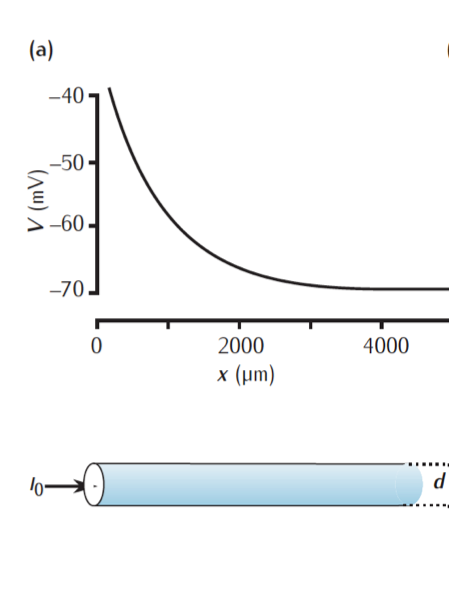
\includegraphics[width=0.7\textwidth]{Figures/Neuron/Semiinf.png}
\end{center}
\caption{\textbf{Semi-infinite cable receiving input $I_e$ in sealed end at $x=0$.} Parameters are $d = 1$ $\mu$m, $R_a=35.4$ cm, $R_m = 10$ m$\Omega$cm$^2$, which gives a length constant $\lambda = 840\, \mu$m. }
\label{Neuron:fig:Semiinf}
\end{figure}

At steady-state, Eq. \ref{eq:cable2} becomes:
\begin{equation}
0 = E_m-\phi_m +  \lambda^2 \frac{\partial^2 \phi_m}{\partial x^2}, 
\label{eq:semiinf}
\end{equation}
at all points along the cable, except $x=0$, where there is the additional injected current, which we will deal with later. If we introduce the new variable $\Delta{phi_m}=\phi_m-E_m$, Eq. \ref{eq:semiinf} simplifies to:
\begin{equation}
\frac{d^2 \Delta{\phi_m}}{d x^2} -  \frac{1}{\lambda^2} \Delta{\phi_m}=0, 
\label{eq:semiinf2}
\end{equation}
which has the solution:
\begin{align}
\Delta{\phi_m}(x) &= \Delta{\phi_m}(0) e^{-x/\lambda} \\
\phi_m(x) &= E_m + \big( \phi_m(0)-E_m \big) e^{-x/\lambda}.
\label{eq:semiinf3}
\end{align}
The (general-solution) term containing $e^{+x/\lambda}$ was excluded from the solution on the count of being unphysical as it diverges when $x \rightarrow \infty$.The injected current will determine what $\phi_m(0)$ is a the boundary, and we may introduce it by defining the input resistance in steady state as $R_{\infty} =  \Delta \phi_m/I_e =  (\phi_m(0)-E_m)/I_e$, according to Ohm's law. With this, Eq. \ref{eq:semiinf3} can be written:
\begin{equation}
\phi_m(x) = E_m + R_{\infty} I_e e^{-x/\lambda}
\label{eq:semiinf4}
\end{equation}

Eq. \ref{eq: semiinf4} is useful as it gives us analytical insight into signals spreading in e.g., passive dendrites. It tells us that in steady-state, the amplitude will decay exponentially from the injection site and outwards, and will be reduced by a factor $1/e$ over the length $\lambda$. If we put in some typical values in eq. \ref{eq:lengthconst}, like a dendritic diameter $d=1$~$\mu$m, a membrane resistance of $R_m=10\;\text{k}\Omega\text{cm}^2$, and an axial resistivity $R_a=35.4\;\Omega\text{cm}$, we would get a length constant of $\lambda = 840\; \mu$m. 

Eq. \ref{eq:lengthconst} also sows that $\lambda \propto \sqrt{d}$, meaning that signals will spread further the thicker the dendrite, and that $\lambda \propto \sqrt{R_m/R_a}$ meaning that the signal is facilitated by having a large membrane resistance compared to the axial resistance. We may also get some insight in what aspects of the neurite that determine the input resistance $R_{\infty}$ by requiring that the axial current at $x=0$ should be identical to the input current. From that, we can calculate the input resistance, 

\begin{align}
&- \frac{4R_a}{\pi d^2} \frac{\partial \phi_m}{\partial x}  = i_e  \Big|_{x=0} \\
&\frac{4R_a \lambda}{\pi d^2} R_{\infty} i_e  = i_e \\
&R_{\infty} =  \sqrt{\frac{4R_m R_a}{\pi^2 d^3}}, 
\label{eq:inputresistance}
\end{align}

where we used eq. \ref{eq:semiinf3} for $\phi_m$ and eq. \ref{eq:lengthconst} for $\lambda$. Eq. \ref{eq:inputresistance} shows that the input resistance is proportional to $1/d^{3/2}$, i.e., the input resistance is higher the thinner the dendrite. 


\subsubsection{\orange{Temporal solutions of cable equation}}
\ghnote{Have to consider what to include here ... what do we want with it? what do we need for later?}
It can be shown that the temporal solution for $\phi_m$ in a passive cable is \cite{rall1969}:
\begin{equation}
\phi_m(x,t) = C_0(x) e^{-t/\tau_0} + C_1(x) e^{-t/\tau_1} + \ldots, 
\label{eq:cabletemporal}
\end{equation}
where the coefficients $C_n(x)$ depend on the distance along the cable, while $\tau_0 = \tau_m = R_m C_m$ is the \emph{membrane time constant}, and the other time constants have successively smaller values ($\tau_0 > \tau_1 > \tau_2 > \ldots$). Fig. \ref{Neuron:fig:temporalrall} shows the the membrane potentials at selected positions along a $500 \, \mu$m long cable responding to a current injection (top panel) resembling a synaptic input in one end. We see that the peak response comes faster in proximal than in distal location, but that potential is about the same at all points along the cable after 2 ms. After this, $\phi_m$  decay gradually towards the resting state. This takes place at the slower time scale of the membrane time constant, which in this simulation was 10~ms ($R_m=1\,\Omega \text{m}^2$, and $C_m=1\,\mu\text{F}/\text{cm}^2$). Although the dynamics of course will be system specific, depending on the membrane time constant and generally on the presence of active mechanisms, the simulation in Fig. \ref{Neuron:fig:temporalrall} may give some general idea on how signals spread in dendrites.

\begin{figure}[!ht]
\begin{center}
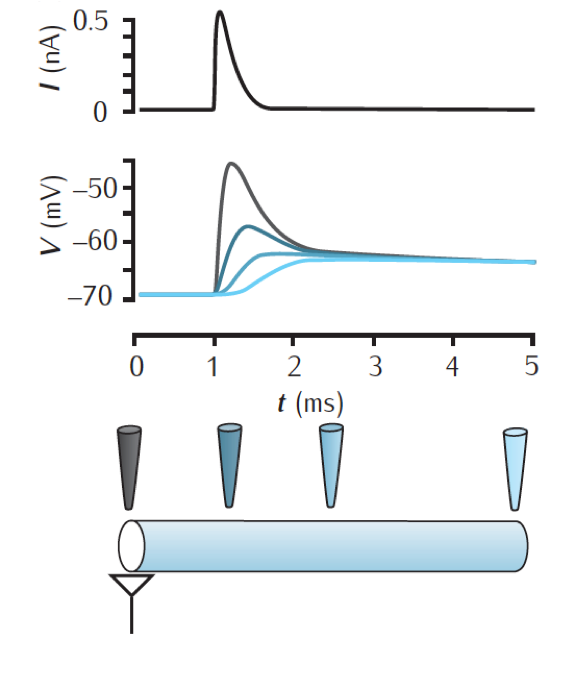
\includegraphics[width=0.7\textwidth]{Figures/Neuron/Temporalcable.png}
\end{center}
\caption{\textbf{Temporal solution of cable equation.}
}
\label{Neuron:fig:temporalrall}
\end{figure}

\subsection{\red{Maybe a subsection about $\lambda$, frequency dependence etc.}}


\subsection{\red{Assumptions}}
\ghnote{Skrive om konsentrasjonseffekter. Tror det er bra aa spare Nernst-potensialene til dette delkap. Si noe om at man ofte ikke trenger aa holde styr paa konsentrasjoner pga. homeostatiske mekanismer "bakt inn" i passiv lekkasje.Si noe om hva som skal til for faktisk aa modellere konsentrasjoner uten aa gaa inn i detalj. Referere til rammeverkene som kommer i Kap 6.}
